\subsection{$n$D-Sphere-geodesic-line picking}
\label{sec:nsphere_geodesic_line}

Sphere-geodesic-line picking is similar to sphere-line picking, except
that the ``lines'' are geodesics on the surface of the sphere, and the
distance metric is the length of these lines.

Can we do this case in general ??? Yes we can all the way down to the circle which gives a uniform distribution.

$n$-Sphere is embedded in $\R^{n+1}$ and encloses the $n+1$-ball


Figures ...

\begin{figure}[tbp]
  \begin{center}
    \subfloat[\label{fig:sphere_geo_eg}Example.]
       {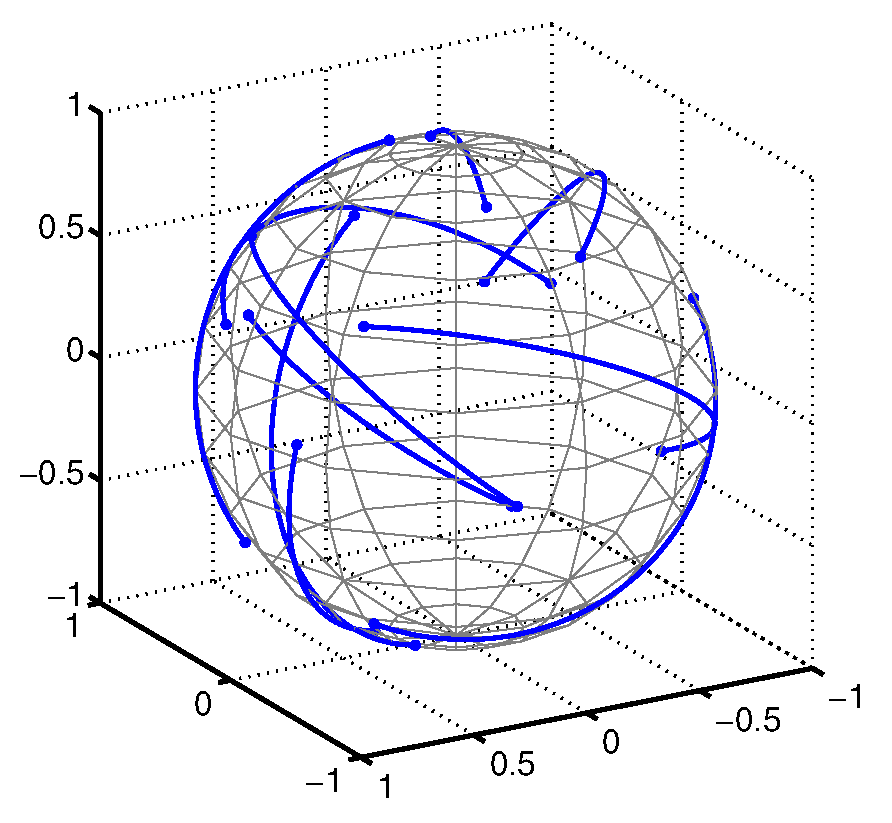
\includegraphics[width=0.4\columnwidth]{../Matlab/Plots/LinePicking_eg_sphere_geodesic.eps}} 
    \hspace{6mm}
    \subfloat[\label{fig:sphere_geo_pdf}PDF.]
       {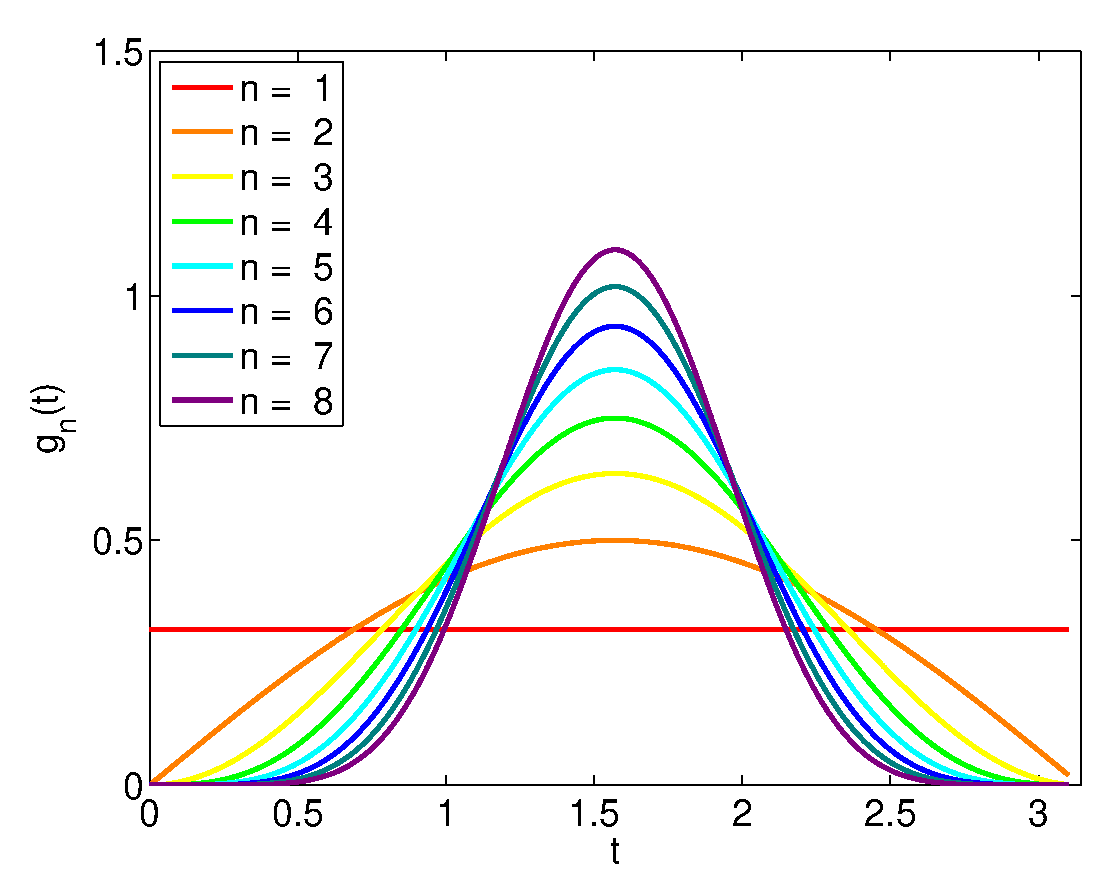
\includegraphics[width=0.48\columnwidth]{../Matlab/Plots/LinePicking_plot_nspheres_geodesic.eps}}
    \caption{The sphere-geodesic-line picking problem.}
  \end{center} 
\vspace{-4mm}
\end{figure}



\subsubsection{PDF}

Obviously, the sphere has spherical symmetry, but as a result, we can,
without loss of generality, assume the first point lies at the pole of
the sphere.

As in the $n$-Sphere above we first determine a density $f(\phi_1)$ function for $\phi_1$ then using the transform method. In fact $f(\phi_1)$ is exactly the same function as in the  $n$-Sphere thus we have:

\begin{equation}  
 f(\phi_1) = \frac{\Gamma\left(\frac{1+n}{2}\right) \sin(\phi )^{n - 1}}{\sqrt{\pi } \Gamma\left(\frac{n}{2}\right)}
\end{equation} 

We have have a function for $d$ the distance between two points in terms of $\phi_1$ so we can get  $\phi_1$ in terms of $d$ thus:

\begin{eqnarray}
  d & = & \phi_1  R.\\
\phi_1& = & \frac{d}{R}\\ 
   \frac {d \frac{d}{R}}{dd} & = & \frac{1}{R}\\
\end{eqnarray}



If $y = g(X)$ then the transform rule  is :  

\[ f_Y(y) = \left| \frac{d}{dy} \left( g^{-1}(y) \right) \right|
                f_X\left( g^{-1}(y) \right)
\]

thus 
\begin{eqnarray}
g_{R}^{n}(d) & = &  \left|\frac{1}{R}\right|  f\left(\frac{d}{R} \right)\\
            & = &   \frac{\Gamma\left(\frac{1+n}{2}\right) 
                            \sin\left(\frac{d}{R}\right)^{n-1}}
                        {\sqrt{\pi } R \Gamma\left(\frac{n}{2}\right)}
\end{eqnarray}

% Using~\eqref{eq:gamma_rel}
% \begin{equation}
%  2^{-(n-1)}\sqrt{ \pi } \Gamma\left[n\right]=\Gamma\left[\frac{n+1}{2}\right] \Gamma\left[\frac{n}{2}\right].  
%   \label{}
% \end{equation}


\subsubsection{CDF}
\begin{equation}
G_{R}^{n}(d)=\frac{1}{2}-\frac{\cos\left(\frac{d}{R}\right) \sin\left(\frac{d}{R}\right)^n \left(\sin\left(\frac{d}{R}\right)^2\right)^{-n/2}\Gamma\left(\frac{1+n}{2}\right) {}_{2}F_{1}\left(\frac{1}{2},1-\frac{n}{2},\frac{3}{2},\cos\left(\frac{d}{R}\right)^2\right) }  {\sqrt{\pi } \Gamma\left(\frac{n}{2}\right)}
\end{equation}

\subsubsection{Moments}

We derive the moments for the case $R=1$ to simplify calculations
(the usual generalization to radius $R$ will be provided at the
end). As usual, the $k$th moment is given by
\begin{eqnarray}
 E[X_{n,1}^k] & = & \int_0^{\pi} 
                    s^k g_{n,1}^{n\mbox{-sphere geo}}(s)
                   \, ds \nonumber \\
      & = & \frac{\Gamma\left(\frac{1+n}{2}\right) }
                 {\sqrt{\pi } \Gamma\left(\frac{n}{2}\right)}
            \int_0^{\pi} 
                    s^k  \sin^{n-1}(s)
                   \, ds
  \label{eq:kth_moment_nsphere_geo}
\end{eqnarray}
For $n=1$ and $k \geq 1$ the integral above is simply
\begin{eqnarray}
 E[X_{1,1}^k] & = & \frac{\Gamma\left(\frac{1+n}{2}\right) \pi^{k+1}}
                 { \sqrt{\pi } \Gamma\left(\frac{n}{2}\right) (k+1)}
        = \frac{\pi^{k}}{k+1}.
\end{eqnarray}
or 
\begin{eqnarray}
 E[X_{1,1}^k] & = &  \frac{\pi^{k} R^k}{k+1}.
\end{eqnarray}

\noindent 
For $n=2$ use \cite[2.633,1.(p.183)]{GandR}
\begin{equation}
  \label{eq:x^n_sin}
  \int x^k \sin(ax) \, dx = - \sum_{i=0}^{k} i! \dbinom{k}{i}
                               \frac{x^{k-i}}{a^{i+1}}
                               \cos\left( ax + i \pi/2 \right).
\end{equation}
For $k=1$ and $2$ we get
\begin{eqnarray}
 E[X_{2,1}^1]
      & = & \frac{\Gamma\left(3/2\right) }
                 {\sqrt{\pi } \Gamma\left(1\right)}
            \left[ -x \cos(x) - \cos(x + \pi/2) \right]_0^{\pi}  \nonumber \\
      & = &  \frac{1}
                 {2}
            \pi,             
             \label{eq:starting_n=1}         \\
 E[X_{2,1}^2] 
      & = & \frac{\Gamma\left(3/2\right) }
                 {\sqrt{\pi } \Gamma\left(1\right)}
            \left[- x^2 \cos(x) - 2 x \cos(x + \pi/2) - 2 \cos(x + \pi) \right]_0^{\pi} \nonumber  \\
      & = & \frac{1}
                 {2}
            \left[ \pi^2  - 4 \right]. 
            \label{eq:starting_n=2}
\end{eqnarray}
For $k=1$ (i.e., calculation of the mean) and general $n$ we use \cite[3.821,1.(p.446)]{GandR}
\begin{equation}
  \label{eq:sin_x_x}
  \int_0^\pi x \sin^{n-1} x \, dx =
       \frac{\pi^2}{2^{n}} \, \frac{\Gamma(n)}{ \Gamma\left((n+1)/2 \right)^2 }, \mbox{ for } n>0.
\end{equation}
The result can ber rearrange with the help of \eqref{eq:gamma_rel} to give
\begin{eqnarray}
 E[X_{n,1}^1]
      & = & \frac{\Gamma\left(\frac{1+n}{2}\right) }
                 {\sqrt{\pi } \Gamma\left(\frac{n}{2}\right)}
            \int_0^{\pi} 
                    s  \sin^{n-1}(s)
                   \, ds \nonumber \\
      & = & \frac{\Gamma\left(\frac{1+n}{2}\right) }
                 {\sqrt{\pi } \Gamma\left(\frac{n}{2}\right)}
              \frac{\pi^2}{2^{n}} \, \frac{\Gamma(n)}{ \Gamma\left((n+1)/2 \right)^2 }
            \nonumber \\
      & = & \frac{\pi^2 \Gamma(n)}
                 {\sqrt{\pi} 2^{n} \Gamma\left(\frac{n}{2}\right) \Gamma\left((n+1)/2 \right)}
            \nonumber \\
      & = & \frac{\pi}{2}.
\end{eqnarray}
In the general case, we multiply by $R$ to get the mean
\begin{eqnarray}
  \label{eq:mean_nsphere_geo}
 E[X_{n,1}^1] & = &  \frac{\pi R}{2}.
\end{eqnarray}
The mean can also be derived directly from symmetry (noting that PDF
is symmetric around $t = \pi R/2$)



Now from \cite[2.631,2.(p.183)]{GandR}
\begin{equation}
  \int x^k \sin^{n-1} (x) \, dx 
   = \frac{x^{k-1} \sin^{n-2}(x)}{(n-1)^2} \left[ m \sin x - (n-1) x \cos x \right]
     + \frac{n-2}{n-1} \int x^k \sin^{n-3}(x) \, dx
     - \frac{k(k-1)}{(n-1)^2} \int x^{k-2} \sin^{n-1} x \, dx 
\end{equation}
Define the integral
\begin{equation}
  \label{eq:m_n-1}
  M(n) = \int_0^\pi x^2 \sin^{n-1} (x) \, dx 
\end{equation}
Take $m=2$ and $n>2$, and integrate from 0 to $\pi$ using \eqref{eq:int_sin_n} and we get
\begin{eqnarray}
 M(n)  & = & \left[ \frac{x \sin^{n-2}(x)}{(n-1)^2} \left[ m \sin x - (n-1) x \cos x \right] \right]_0^\pi
        + \frac{n-2}{n-1} M(n-2)
        - \frac{2}{(n-1)^2} \int_0^\pi \sin^{n-1} x \, dx 
            \nonumber \\
 & = & \frac{n-2}{n-1} M(n-2)  - \frac{2}{(n-1)^2} \frac{\sqrt{\pi} \, \Gamma\big( n/2 \big)}{\Gamma\big( (n+1)/2 \big)}.
\end{eqnarray}
The second moments for $n>2$ are therefore given by
\begin{eqnarray}
 E[X_{n,1}^2]
      & = & \frac{\Gamma\left(\frac{1+n}{2}\right) }
                 {\sqrt{\pi } \Gamma\left(\frac{n}{2}\right)}
            M(n) \nonumber \\
       & = & \frac{\Gamma\left(\frac{1+n}{2}\right) }
                 {\sqrt{\pi } \Gamma\left(\frac{n}{2}\right)}
            \left[   \frac{n-2}{n-1} M(n-2) 
                     - \frac{2}{(n-1)^2} \frac{\sqrt{\pi} \, \Gamma\big( n/2 \big)}{\Gamma\big( (n+1)/2 \big)} \right] \nonumber \\
       & = & \frac{\Gamma\left(\frac{1+n}{2}\right) }
                 {\sqrt{\pi } \Gamma\left(\frac{n}{2}\right)}
              \frac{n-2}{n-1} M(n-2) 
                     - \frac{2}{(n-1)^2}  \nonumber \\
     & = & E[X_{n-2,1}^2] - \frac{2}{(n-1)^2},
\end{eqnarray}
where we note that $\Gamma(z) = (z-1) \Gamma(z-1)$.  So we now have a
recursion for the general case, starting with the $n=1$ and $2$ values
given in \eqref{eq:starting_n=1} and \eqref{eq:starting_n=2},
respectively. 
\begin{eqnarray}
  \label{eq:mean_nsphere_geo}
  E\big[ X_{1,R}^2 \big] & = & R^2 \frac{\pi^2}{3}, \\ 
  E\big[ X_{2,R}^2 \big] & = & R^2 \left( \frac{\pi^2}{2} - 2 \right), \\ 
  E\big[ X_{n,R}^2 \big] & = & E\big[ X_{n-2,R}^2 \big] 
                                   - \frac{2 R^2}{(n-1)^2}, \;\;\;
                                   \mbox{ for } n > 2.
\end{eqnarray}
or we can directly calculate the variances
\begin{eqnarray}
  \label{eq:mean_nsphere_geo}
  Var\big[ X_{1,R} \big] & = & R^2 \frac{\pi^2}{3} - E\big[ X_{1,R} \big]^2, \nonumber\\ 
              & = & R^2 \frac{\pi^2}{12}, \nonumber\\ 
  Var\big[ X_{2,R} \big] & = &  R^2 \left( \frac{\pi^2}{2} - 1 \right) - E\big[ X_{2,R} \big]^2 \nonumber\\ 
               & = & R^2\left(  \frac{\pi^2}{4} - 2 \right), \nonumber\\ 
  Var\big[ X_{n,R} \big] & = & Var\big[ X_{n-2,R} \big] 
                                   - \frac{2 R^2}{(n-1)^2}, \;\;\;
                                   \mbox{ for } n > 2.\nonumber
\end{eqnarray}
because $E\big[ X_{n,R} \big] = \pi R /2$ for all $n$.  We push back
to the case $n=0$ for elegance of notation: 
\begin{eqnarray}
  \label{eq:mean_nsphere_geo}
  Var\big[ X_{0,R} \big] & = & R^2 \frac{\pi^2}{4}, \\ 
  Var\big[ X_{1,R} \big] & = & R^2 \frac{\pi^2}{12}, \\ 
  Var\big[ X_{n,R} \big] & = & Var\big[ X_{n-2,R} \big] 
                                   - \frac{2 R^2}{(n-1)^2}, \;\;\;
                                   \mbox{ for } n > 1.
\end{eqnarray}
Written as a summation
\begin{eqnarray}
  \label{eq:mean_nsphere_geo}
  Var\big[ X_{n,R} \big] & = & R^2 \times \left\{ \begin{array}{ll}
      \displaystyle
         \frac{\pi^2}{12} 
        - 2 \sum_{k=1}^{(n-1)/2} \frac{1}{(2k)^2}, & 
          \mbox{ for $n$ odd,} \\ 
      \displaystyle
          \frac{\pi^2}{4} 
        - 2 \sum_{k=1}^{n/2} \frac{1}{(2k-1)^2}, &
          \mbox{ for $n$ even,} \\ 
    \end{array} \right.
\end{eqnarray}
where the summation terms are understood to be zero for $n=0, 1$.

Now from \cite[0.234,2.(p.7)]{GandR} and \cite[0.233,3.(p.7)]{GandR}  we get
\begin{eqnarray}
  \sum_{k=1}^{\infty} \frac{1}{(2k-1)^2} & = & \frac{\pi^2}{8},  \\
  \sum_{k=1}^{\infty} \frac{1}{(2k)^2}
%            & = & \frac{2 \pi^2}{2} |B_2| - \frac{\pi^2}{8},
           & = &  \sum_{k=1}^{\infty} \frac{1}{k^2} - \sum_{k=1}^{\infty} \frac{1}{(2k-1)^2}, \nonumber \\
           & = & \frac{\pi^2}{6}  - \frac{\pi^2}{8}  , \nonumber \\
           & = & \frac{\pi^2}{24} ,
\end{eqnarray}
so the limiting forms of the variance for large $n$ are both
zero. Given the density integrates to one, but has variance
approaching zero for large $n$, it is reasonable to think of it as a
delta-function for large $n$. In this case, it would be natural to
think of it as a deterministic distribution, i.e., when the number of
dimensions are large, then every pair of random points is roughly the
same distance apart. Does this make sense at all?

% B_2 = Bernoulli number = 1/6, G&R, 9.61 or 
% http://en.wikipedia.org/wiki/Bernoulli_number
%   



